\documentclass[a4paper,12pt]{report}
\usepackage[utf8]{inputenc}
\usepackage[francais]{babel}
\usepackage{fancyhdr}
\usepackage{graphicx}
\usepackage{tikz}
\usetikzlibrary{calc}
\usepackage{listings}
\usepackage{color}
\usepackage{xcolor}
\definecolor{grey}{rgb}{0.9,0.9,0.9}
\usepackage{titlesec}
\usepackage{verbatim}
\usepackage{listings}
\usepackage{textcomp}
\usepackage{hyperref}
\usepackage{ amssymb }


\lstset{
language=Java, basicstyle=\footnotesize, 
  numbers=left,         
  numberstyle=\tiny\color{gray}, 
  stepnumber=1, 
  numbersep=5pt,                  
  backgroundcolor=\color{white},  
  showspaces=false,               
  showstringspaces=false,         
  showtabs=false,                 
  frame=single,                   
  rulecolor=\color{black},        
  tabsize=2,                      
  captionpos=b,                   
  breaklines=true,                
  breakatwhitespace=false,        
  title=\lstname,           
keywordstyle=\color[rgb]{0,0,1},
commentstyle=\color[rgb]{0.133,0.545,0.133},
stringstyle=\color[rgb]{0.627,0.126,0.941},
}

\frenchbsetup{StandardLists=true}
\newcommand{\marge}{18mm}
\usepackage[left=\marge,right=\marge,top=\marge,bottom=\marge]{geometry}
\pagestyle{fancy}
\setlength{\headheight}{14pt}
\chead{
  \textbf{Binôme :} Douaille Erwan \& Yanis Nait Abdelaziz
  \hspace{2em}
  \textbf{Groupe :} M1 Info TI}
\renewcommand{\headrulewidth}{1pt}
\linespread{1}
\setlength{\columnseprule}{0.2pt}



\begin{document}


\makeatletter
\begin{titlepage}
\centering
\vspace{-10em}
{\LARGE \textbf{\textsc{Rapport de Projet RVI}}}\\
\vspace{3em}

\includegraphics[scale=0.6]{image/thalassa.png}\\
\vspace{3em}
{\LARGE \textsc{Projet Thalassa: simulation de plongée sous-marine}}\\

\vspace{8em}
Par\\
\vspace{1em}
{\LARGE \@author}\\

\vspace{2em}



\begin{tikzpicture}[remember picture,overlay]

\node [below left,xshift=-1cm, yshift=4cm] at (current page.south east){
\includegraphics[scale=0.6]{image/ustl1.png}};

\end{tikzpicture}
\end{titlepage}
\makeatother

\sloppy

\setcounter{page}{1} 
\newpage

%%%%%%%%%%%%%%%%%%%%%%%%%%%%%%%%%%%% INTRODUCTION
%%%%%%%%%%%%%%%%%%%%%%%%%%%%%%%%%%%%%%%%%%%%%%%%%
%%%%%%%%%%%%%%%%%%%%%%%%%%%%%%%%%%%%%%%%%%%%%%%%%
\section*{Introduction}

Dans ce compte rendu nous allons voir comment appliquer des modifications sur les pixels; faire des corrections sur les niveaux de gris, répartir les valeurs de 0 à 255 et appliquer des modifications sur la LUT (Look up table), table servant à faire la conversion donnée de l'image lue et rendu visuel.
	
\section*{Question 1}

\begin{lstlisting}macro "q1"{
	image = getImageID();
	
	width= getWidth();
	height= getHeight();

	min=255;
	max=0;

	// Recherche du minimum et maximum
	for(j=0;j<height;j++){
		for(i=0;i<width;i++){
			p=getPixel(i,j);
			if(p<min)
				min=p;
			if(p>max)
				max=p;
		}
	}
	print("min = ",min);
	print("min = ",max);
	
	// declaration des LUTs
	taille=256;
    reds = newArray(taille); 
    greens = newArray(taille); 
    blues = newArray(taille);

	// Recuperation des LUTS
    getLut(reds, greens, blues);
	
	b=255/(max-min);
	a=-b*min;
	
	//Correction affine
	for(i=0;i<taille;i++){
		reds[i]=a+(b*reds[i]);
		greens[i]=a+(b*greens[i]);
		blues[i]=a+(b*blues[i]);
	}
	
	//Mise a jour de la lut
	setLut(reds, greens, blues);
\end{lstlisting}

Nous avons obtenu comme minimum 35 et 240 en maximum. Grâce à l'application de la fonction affine l'image semble plus dynamique, moins terne.

\newpage
	
\section*{Question 2}


\begin{figure}[!ht]
	\center
	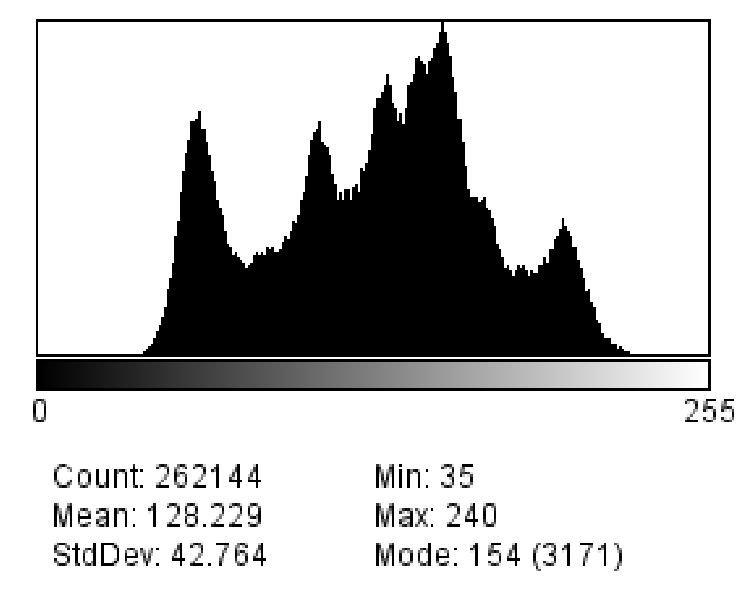
\includegraphics[scale=0.4]{image/histo_base.png}
	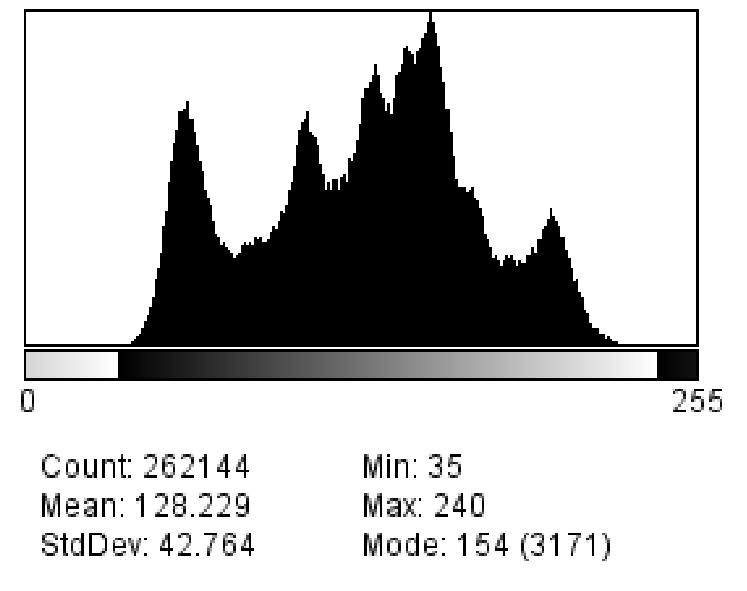
\includegraphics[scale=0.4]{image/histo_correction_affine.png}
\end{figure}

Si on compare les deux histogrammes pour les deux images, on constate qu'ils sont identiques malgrès que l'aspect visuel des deux images ne soit pas le même.
On peut donc dire que la modification de la LUT n'agit que sur l'aspect visuel de l'image. Dans la question 3 on nous demandera justement d'appliquer notre fonction affine directement sur le niveau de gris des pixels de l'image
	
\section*{Question 3}


\begin{figure}[!ht]
	\center
	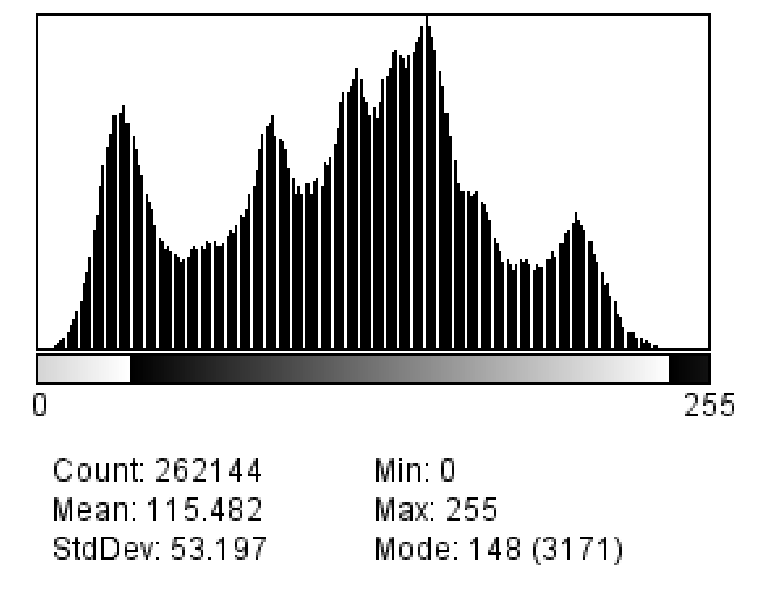
\includegraphics[scale=0.4]{image/histo_q3.png}
	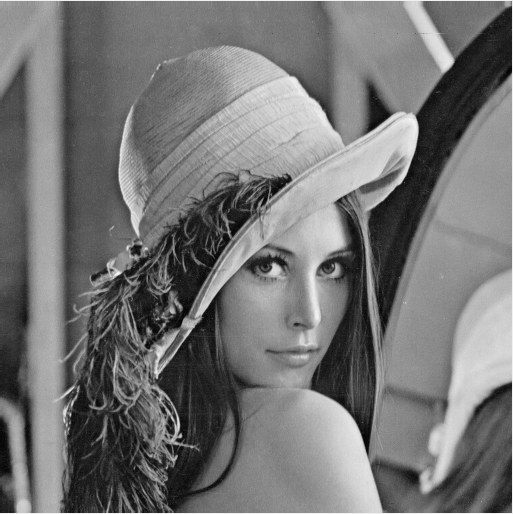
\includegraphics[scale=0.4]{image/image_q3.png}
\end{figure}

\begin{lstlisting}
	\\ question 3	
	\\ rappel 	b=255/(max-min); 	a=-b*min;
	for (j=0; j<height; j++)	{
		for (i=0; i<width; i++){
			p = getPixel(i,j);
			setPixel(i,j,a+b*p);
		}
	}
\end{lstlisting}

Içi on applique notre fonction affine à toutes les pixels de l'image.

\newpage
	
\section*{Question 4}


\begin{figure}[!ht]
	\center
	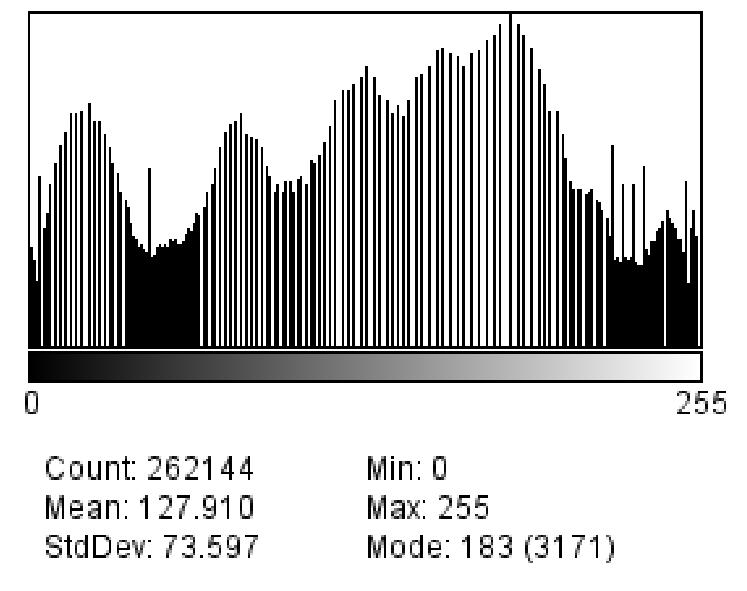
\includegraphics[scale=0.4]{image/histo_egalise.png}
	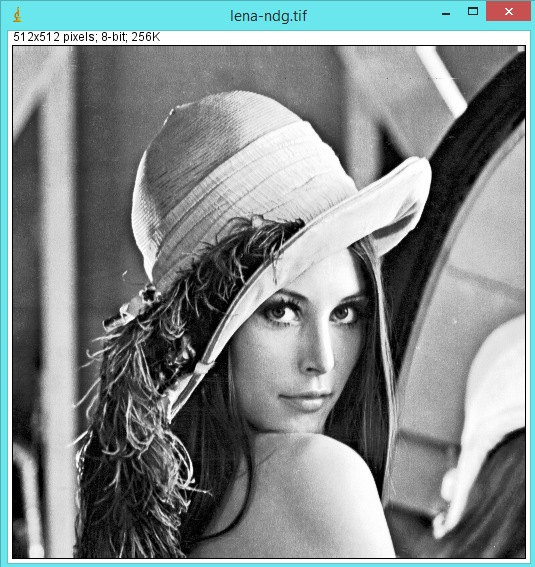
\includegraphics[scale=0.4]{image/image_q4.png}
\end{figure}

\begin{lstlisting}
  EgalisationHistogramme();
  function EgalisationHistogramme(){
		image = getImageID();
	
		width= getWidth();
		height= getHeight();
		N=height*width;
		
		\\on compte tout les pixels
		bins = 256;
		getHistogram(values, counts, bins);
		histoCumule = newArray(256);
		histoCumule[0]=counts[0];
		for(i=1;i<256;i++){
			histoCumule[i]=counts[i]+histoCumule[i-1];
			//print(histoCumule[i]);
		}
		
		\\on affecte les pixels
		for(j=0;j<height;j++){
			for(i=0;i<width;i++){
				p=getPixel(i,j);
				//print(" ,",p);
				c=(histoCumule[p]*255)/N;
				setPixel(i,j,c);
			}
		}
  }
\end{lstlisting}

En visualisant l'histogramme on observe que les niveaux de gris des pixels va de 0 à 255. L'égalisation a permis d'harmoniser l'histogramme et le nombre d'occurences des pixels s'est étalé de 0 à 255.

Cette méthode permet d'obtenir une image plus claire, le contraste est plus élevé.
	
\newpage
	
\section*{Conclusion}

Nous avons vu dans ce travaux pratiques comment modifier l’aspect visuel d’une image sans modifier l’histogramme (en modifiant la Look Up Table) et en modifiant l’histogramme(en travaillant directement sur le niveau de gris du pixel).

Nous avons également appliqué deux types de transformations. L'une permettant de rendre l'image moins terne grâce à la fonction de correction affine et l'autre méthode, l'égalisation de l'histogramme qui nous à permis d'obtenir une image plus claire.

\end{document}
